\documentclass[11pt]{article}

% basic packages
\usepackage[margin=1in]{geometry}
\usepackage[pdftex]{graphicx}
\usepackage{amsmath,amssymb,amsthm}
\usepackage{custom}
\usepackage{lipsum}
\usepackage{hyperref}
\usepackage{fancyvrb}
\usepackage{tcolorbox}

% page formatting
\usepackage{fancyhdr}
\pagestyle{fancy}

\renewcommand{\sectionmark}[1]{\markright{\textsf{\arabic{section}. #1}}}
\renewcommand{\subsectionmark}[1]{}
\lhead{\textbf{\thepage} \ \ \nouppercase{\rightmark}}
\chead{}
\rhead{}
\lfoot{}
\cfoot{}
\rfoot{}
\setlength{\headheight}{14pt}

\linespread{1.03} % give a little extra room
\setlength{\parindent}{0.2in} % reduce paragraph indent a bit
\setcounter{secnumdepth}{2} % no numbered subsubsections
\setcounter{tocdepth}{2} % no subsubsections in ToC

\begin{document}

% make title page
\thispagestyle{empty}
\bigskip \
\vspace{0.1cm}

\begin{center}
{\fontsize{22}{22} \selectfont Notes on}
\vskip 16pt
{\fontsize{20}{20} \selectfont \bf \sffamily Natural Language Processing}
\vskip 24pt
{\fontsize{18}{18} \selectfont \rmfamily Mann Malviya}
\vskip 6pt
{\fontsize{14}{14} \selectfont \ttfamily {\hypersetup{urlcolor=black}\href{mailto:mannmalviya15@gmail.com}{mannmalviya15@gmail.com}}}
\vskip 24pt
\end{center}

{\parindent0pt \baselineskip=15.5pt These notes provide an introduction to Natural Language Processing. The primary sources used to write these notes were:

\begin{itemize}
    \item CSE 143: Natural Language Processing — UCSC
    \item Textbook for the course: Speech\& Language Processing (3rd Edition preprint) -- Jurafsky \& Martin
    \item Textbook for the course: Natural Language Processing -- Jacob Eisenstein's online book

\end{itemize}

Please report any errors to \href{mailto:mannmalviya15@gmail.com}{mannmalviya15@gmail.com}


}

% make table of contents
\newpage
\tableofcontents
\newpage

% main content
\section*{Lecture 1: Introduction}
\addcontentsline{toc}{section}{Lecture 1: Introduction}

\subsection*{Topics \& Course Overview}
\addcontentsline{toc}{subsection}{Topics \& Course Overview}
\begin{itemize}
  \item Introduction to NLP
  \item NLP Applications
  \item Text Classifiers
  \item Language Models
  \item Neural Networks
  \item Sequence Models 
  \begin{itemize}
    \item part-of-speech tagging
    \item named-entity recognition
    \item etc..
  \end{itemize}
  \item Syntax \& Parsing
  \item Pretraining models
\end{itemize}

This class will \textbf{introduce NLP} broadly and talk about some of the \textbf{applications of NLP}, one of them being classifying text(Eg: a email spam classifier). 

\

This class will then spend a lot of time on \textbf{language modelling}(this is also a hot topic currently!). 

\

Then we will talk about \textbf{Neural Networks}, how they work, how to build them and how to use them for NLP tasks(for things like a language model!).

\

We will also talk about some different kinds of \textbf{Sequence models}, there's a lot of tasks you could view in terms of a series of things happening, typically words, a word happens and then another word happens..., you might want to ask questions about that sequence of words, eg: given this words place in this sequence, "what do I know about it?"---disambiguation questions.


For example is the below word in the sentence, wind as in "wind blowing" or "wind the clock".
\begin{center}
\begin{BVerbatim}
"...wind..."
\end{BVerbatim}
\end{center}


The two problems here are:
\begin{enumerate}
  \item word sense disambiguation
  \item part-of-speech tagging  
\end{enumerate}

We treat understanding the meaning of a word in a particular context(\textbf{word sense disambiguation}) as a sequence labeling problem. \textbf{Part-of-speech-tagging} means marking things like nouns, verbs, adjective etc. in a sentence.


Then we will talk a bit about \textbf{syntax} and then understanding the syntax of sentences as we get them. The syntax of a language is like it's structure. The problem of recovering the syntactic structure of a sentence is called \textbf{parsing}.


Finally we will talk about pre-training models!

\subsection*{What is natural language processing?}
\addcontentsline{toc}{subsection}{What is natural language processing?}

\subsubsection{Ok what's natural language?}
Before we answer that, lets start by asking what is not natural language.

A \textbf{formal language} is something that is mathematically defined (eg. something you could do the pumping lemma on), i.e., you've got CFG rules, lambda calculus stuff, nested parentheses etc. If you can write down the complete grammar of the language and then you could answer questions based on that complete grammar, then that would be a formal language. An example of formal language is a programming language(eg: LISP or Rust) or if someone writes down a regular expression that defines a set of strings, that set of strings is a formal language. 



We also have \textbf{constructed languages}(shortform: conlang) (some examples of conlang: Toki Pona, Esperanto, Volapük, ido, lojban and also Klingon\footnote{The Klingon language is the constructed language spoken by a fictional alien race called the Klingons in the Star Trek universe.}, Belter Creole\footnote{Belter Creole (lang Belta) is a constructed language (conlang) developed by linguist Nick Farmer for The Expanse television series, based on, but expanding upon, fragmented words from the books.}, Sindarin\footnote{Sindarin is a constructed Elvish language created by J.R.R. Tolkien, functioning as the primary spoken tongue of Elves and Men in Middle-earth during the Third Age.})

So far we defined natural language, by what it's not. Natural language is a language that people are speaking in practice, i.e., there are(or were) native speakers of it.

% Note / Aside
\begin{tcolorbox}[colback=gray!10, colframe=gray!50, title=Note]
On \href{https://en.wikipedia.org/wiki/Esperanto}{Esperanto} and the question: "Could a constructed language become a natural language?"

In the 1800s \textit{L.L. Zamenhof}, living in Europe, after seeing the diverse set of languages people were speaking, came up with the idea that everybody would speak whatever languages they speak but they would also learn Esperanto, which he specifically constructed to be easy for people who already speak a European language to learn. It is \textbf{NOT} a natural language.


If children are raised speaking a conlang, this would be the \textit{creolization}\footnote{A \textit{creole} forms when two groups of people who don't share a language need to communicate. First they develop a pidgin — a simplified, mixed contact language with no native speakers. When children grow up speaking that pidgin as their first language, it becomes a creole — a fully-fledged natural language with native speakers, complex grammar, and all the expressive power of any other natural language.

Creolization is that process of a pidgin becoming a creole.[this footnote was generated by an llm(Sonnet4.6)]}.
Once there are native speakers of a language. It then starts to become more like a natural language. This is how language evolution happens. 

\end{tcolorbox}


\subsubsection{What does it mean to process it?}
We are going to write computer programs that deal with language. Language can come in a lot of modalities, speech, sign language, writing. Writing is the modality simplest for computers(even though it is the most artificial and it's the newest out of all the other modalities). 


\subsubsection{Why do we want this?}

??

\subsection*{Human language is special!}
\addcontentsline{toc}{subsection}{Human language is special!}

We equate the ability to communicate in human language with \textit{intelligence} lots of animals communicate, but only humans have \textit{grammar} like we do. Very few animals can do \textit{reference, pointing, deixis\footnote{the function or use of deictic words, forms, or expressions. i.e., indicating something else. You could think of it as the "greekified" way of talking about pointing.}}. Humans have specialized hardware in their brain, as a result of evolution, for language, and learning language as a baby.


When we talk about grammar we mean the nested structure of human language, this is completely unique to humans. By nested structure we mean things like: Clauses and parentheticals. A clause is a series of words where you have got a verb and typically a subject for that verb. You can put more clauses inside of a clause, and you can put more clauses inside those nested clauses as well.


Human language can also do reference (refer to that tree for example), but this idea of referencing things is not completely unique to humans, there are animals that can understand pointing and do pointing, like domesticated dogs(there's literally a dog breed called "pointers"). Interestingly the animals that can do pointing seemingly learned it from us, we can make such a claim after looking at the fact that wolves(wild relatives) do not understand or do pointing unlike their domesticated counterparts.[may have to fact-check this last point about animals learning pointing from humans]

\subsection*{We say things and we mean them: semiosis}
\addcontentsline{toc}{subsection}{We say things and we mean them: semiosis}
\begin{figure}[h]
    \centering
    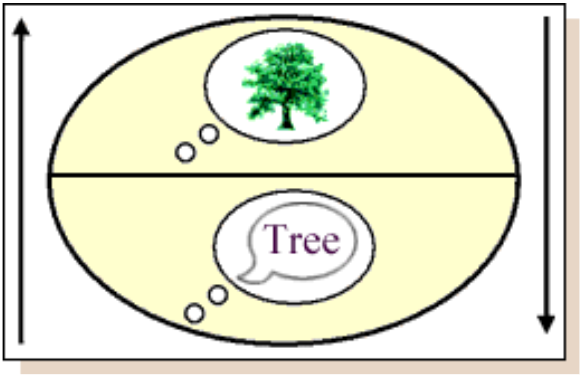
\includegraphics[width=0.5\textwidth]{semiosis.png}
    \caption{"Semiotics for Beginners", \href{https://www.cs.princeton.edu/~chazelle/courses/BIB/semio2.htm}{ Daniel Chandler at Princeton}}
\end{figure}
\begin{itemize}
  \item When you use a word (signifier) it is referring to something (signified).
\end{itemize}

The idea of the relationship between the sign(a word you said) and the signified(the reference in the real world that your word has). Any time you say a noun you are referring to stuff in the world(Eg: desk). 


So the word you say is the \textbf{signifier} and the thing in the world you are referring to is the \textbf{signified}.

\begin{itemize}
  \item Is this possible for a system that's only been trained on text?
\end{itemize}

When you say words, you are also thinking about something as you say those words. There's a debate in the history of AI and our ideas about what it means to build intelligent systems and even building NLP systems broadly. If you have a system that has only been trained on text, then it has signifiers(it has words) but what does it know about those words? 


There's 2 problems here:
\begin{enumerate}
  \item The problem of expecting words.
  \item The problem of words having a referrend in the world
\end{enumerate}

In philosophy this is called the \textbf{symbol grounding problem}. The symbol grounding problem is about how you understand the relationship between a word and the things that it's referring to in the world.


LLMs are trained on just text, the text doesn't refer to anything for the LLM. Even though the LLM doesn't ground that text to things in the real world, it does get other words, i.e., the context, so it knows what other words are likely to come nearby. That's actually all it knows! --- it knows what words happen in what context.

\begin{itemize}
  \item Does that matter?
\end{itemize}

You can have multi-modal AI's that accept videos, images and audio!

\subsection*{The Turing Test}
\addcontentsline{toc}{subsection}{The Turing Test}
\begin{itemize}
  \item So if a machine can use human language, what does that mean?
\end{itemize}

Alan Turing, 1950: If you are having a textual chat conversation with something and you can't tell reliably whether it's a human being or a machine, then that's a pretty good indication that, that machine is intelligent. 


However, LLM powered chatbots are really convincing at passing the Turing test, yet we can make very strong arguments for these things not being particularly intelligent. So we have basically shown that human language is not a sign of a sentient being. These LLM systems lack symbol grounding.




\begin{itemize}
  \item Why can a human be wrong?
  \begin{itemize}
    \item Lying
    \item Misinformed
    \item Misremembering
    \item Bad inference
  \end{itemize}

  \item Why can an LLM be wrong?
  \begin{itemize}
    \item Because it's just predicting what word is most likely to come next\footnote{This is the exact same reason why an LLM is right other times! LLM "hallucinations" are not a thing! The LLM does the same thing when it produces a correct and incorrect output.}
  \end{itemize}
\end{itemize}

\subsection*{Why is NLP hard?}
\addcontentsline{toc}{subsection}{Why is NLP hard?}
NLP is hard because language is hard. One of the most salient ways that language is hard is the built-in ambiguity in the language. You might have different meanings for a individual word, you might have multiple different structural interpretations of a sentence.

\begin{verbatim}
"At last, a computer that understands you like your mother."
\end{verbatim}
Possible interpretations:
\begin{itemize}
  \item A computer that understand you in the way your mother understand you.
  \item A computer that understands the fact that you like your mother.
  \item Then there are multiple more interpretations of this depending on how well your mother understands you, your mother understands you a lot or your mother doesn't understand you.
\end{itemize}

\subsection*{NLP Applications}
We will talk about some NLP applications in this class, like Machine Translation, question answering, search engines.  <FINISH THE LAST 5mins of lecture1>

\vspace{0.5em}
\noindent\rule{\textwidth}{5pt}
\vspace{0.5em}

\newpage

\section*{Lecture 2: More Introduction}
\addcontentsline{toc}{section}{Lecture 2: More Introduction}

\end{document}
